% 일반적인 이미지를 사용하는 부분
%%%%%%%%%%%%%%%%%%%%%%%%%%%%%%%%%%%%%%%%%%%%%%%%%%%%%%%%%%%%%%%%%%%%%%%%%%
bla. \\
    \vspace{-4mm}  
        \begin{figure}[!h]\centering
    		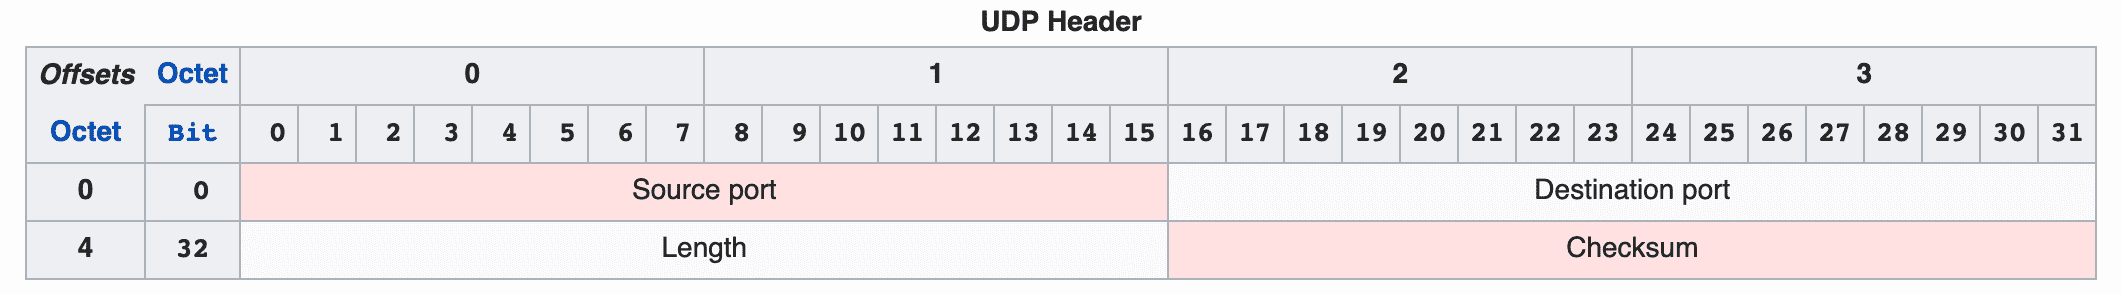
\includegraphics[width=.9\textwidth]{image/week01/2-1.png}
    		\caption{\small UDP Header}
    		\vspace{-10pt}
        \end{figure}
%%%%%%%%%%%%%%%%%%%%%%%%%%%%%%%%%%%%%%%%%%%%%%%%%%%%%%%%%%%%%%%%%%%%%%%%%%
% 떠다니는 figure로 
%%%%%%%%%%%%%%%%%%%%%%%%%%%%%%%%%%%%%%%%%%%%%%%%%%%%%%%%%%%%%%%%%%%%%%%%%%
\vspace{-4mm}  
\begin{wrapfigure}{l}{0.5\textwidth} \vspace{-20pt}
\begin{center}
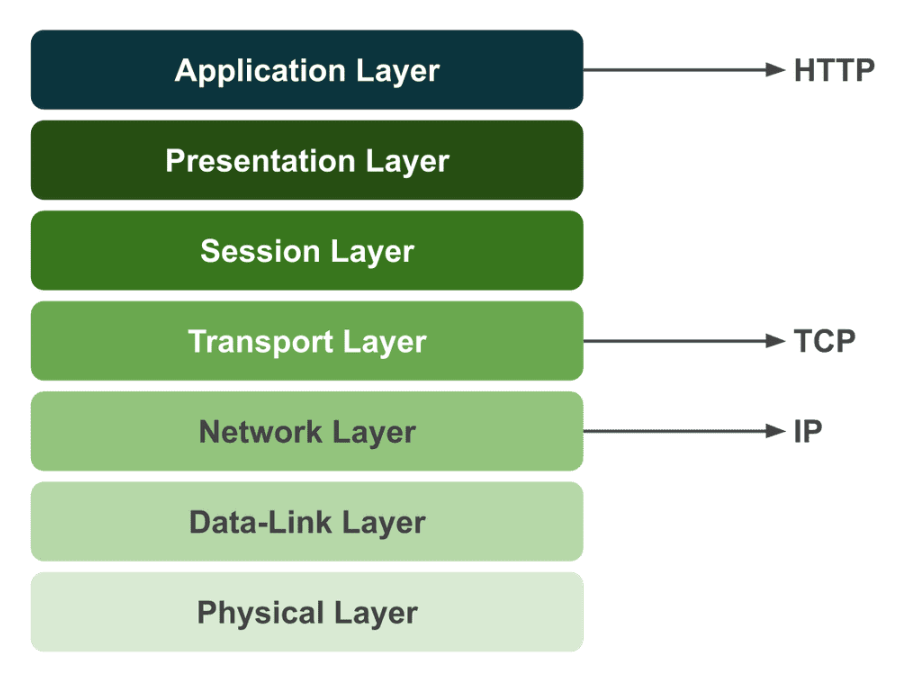
\includegraphics[width=0.43\textwidth]{image/week01/1-0.png}    
\end{center}
\vspace{-20pt}
\caption{\small OSI 7 Layer}
\vspace{-10pt}
\end{wrapfigure}
%%%%%%%%%%%%%%%%%%%%%%%%%%%%%%%%%%%%%%%%%%%%%%%%%%%%%%%%%%%%%%%%%%%%%%%%%%
% subfig 에서 1 X 2 의 이미지를 사용하는 방법
%%%%%%%%%%%%%%%%%%%%%%%%%%%%%%%%%%%%%%%%%%%%%%%%%%%%%%%%%%%%%%%%%%%%%%%%%%
\begin{figure}[h!]
\centering
\subfloat[Distribution of training data. Uncertainty in center of pressure is selected uniformly.]{
    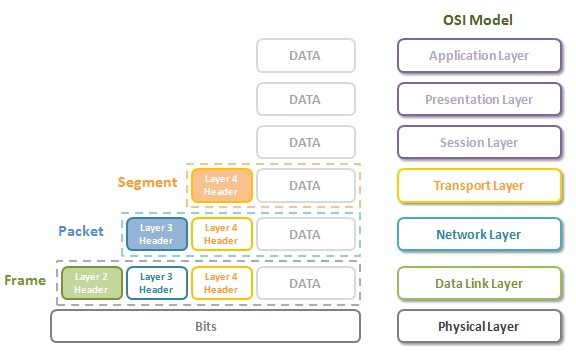
\includegraphics[width=0.2\textwidth] {image/week01/1-2-1.png}
}
\subfloat[Distribution of test data. Uncertainty in center of pressure is selected uniformly.]{
    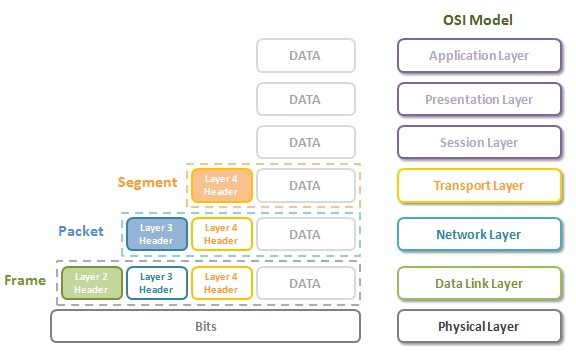
\includegraphics[width=0.5\textwidth] {image/week01/1-2-1.png}
}
\hfill
\subfloat[Distribution of training data. Uncertainty in center of pressure is selected uniformly.]{
    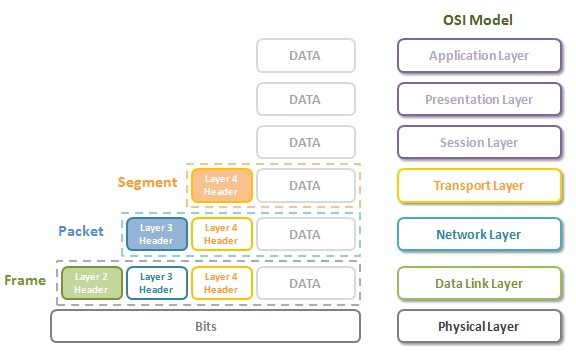
\includegraphics[width=0.2\textwidth] {image/week01/1-2-1.png}
}
\subfloat[Distribution of test data. Uncertainty in center of pressure is selected uniformly.]{
    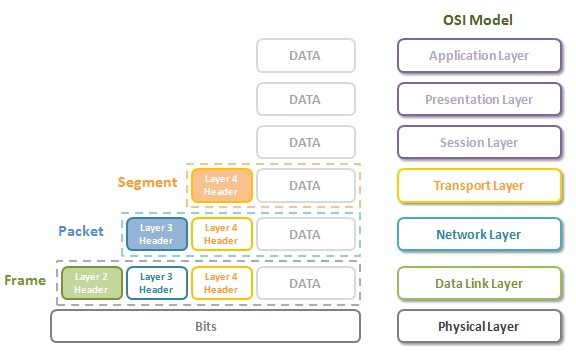
\includegraphics[width=0.5\textwidth] {image/week01/1-2-1.png}
}
\end{figure}
%%%%%%%%%%%%%%%%%%%%%%%%%%%%%%%%%%%%%%%%%%%%%%%%%%%%%%%%%%%%%%%%%%%%%%%%%%